\documentclass{article}
\usepackage{graphicx} % Required for inserting images
\usepackage{hyperref}

\renewcommand{\cite}[1]{[\ref{#1}]}
\renewcommand{\labelenumi}{[\theenumi]}

\begin{document}

\section*{BA Research Notes}

In this bachelor thesis we will try to analyze the mechano-elastic properties of the extracellular fibrous structure of the lymph nodes around germinal centers. 

\subsection*{Lymph Node Structure}

The lymph nodes are split into the outer cortex and the inner medula. The lymph nodes are further compartmentized into so called nodules each includes a part of the cortex with B-cell follicles, a paracortex of T-cells and a part of the medula. 

\begin{figure}[h]
    \centering
    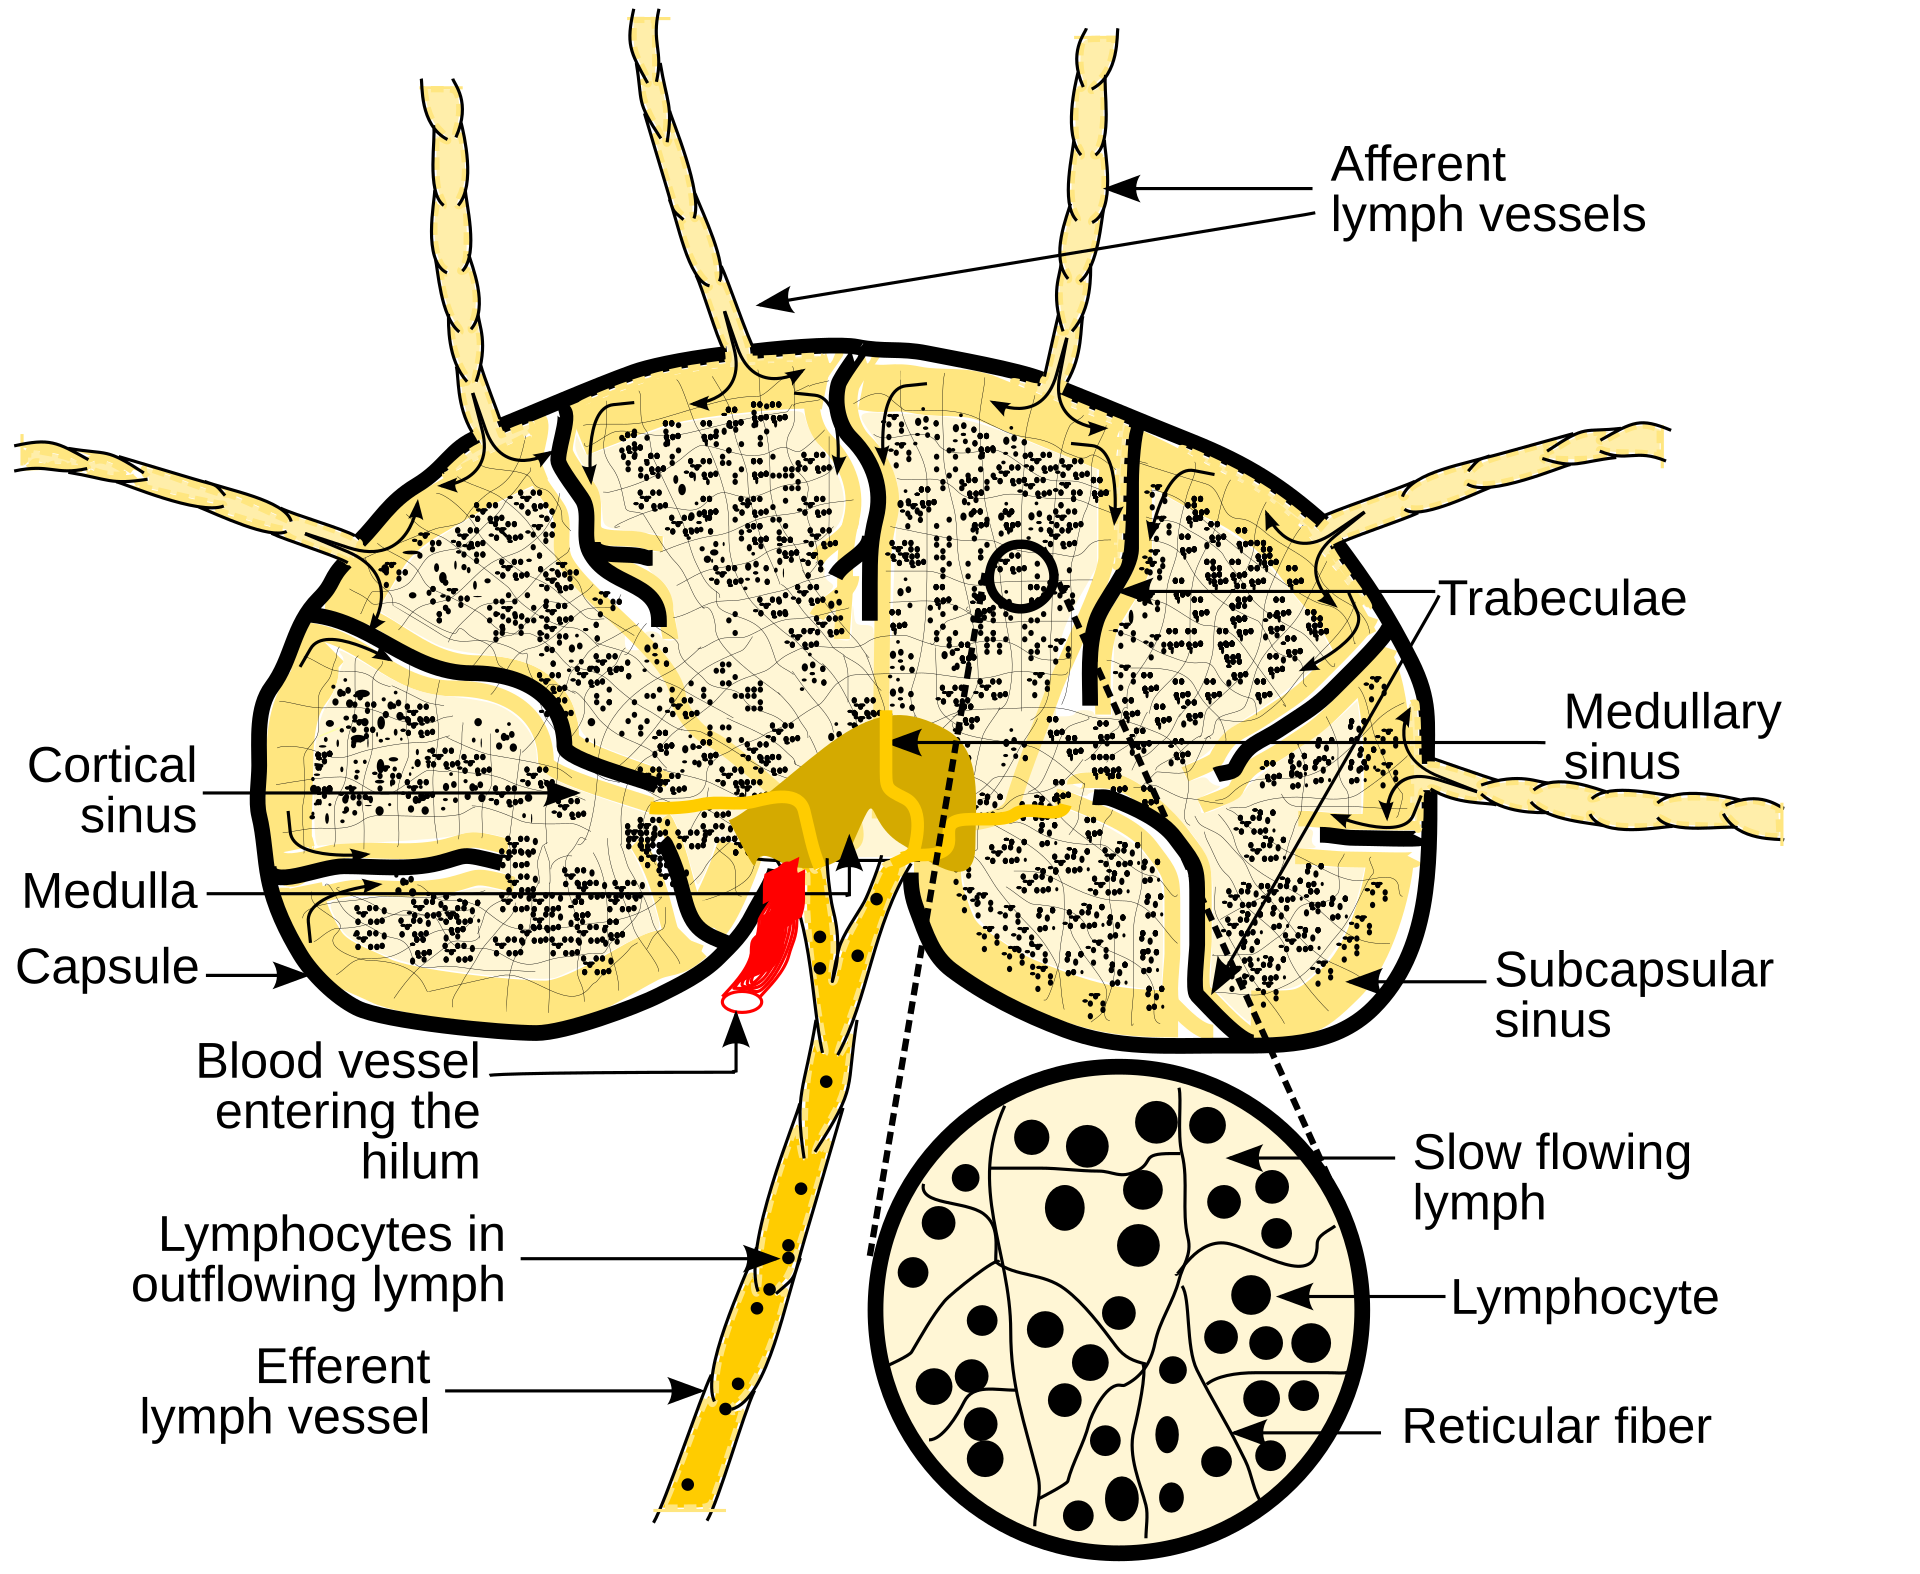
\includegraphics[width=0.5\linewidth]{lymph_node_pic1.png}
    \caption{Picture of the Lymph Node Structure \cite{lymphnode1}}
    \label{fig:lymph_pic_1}
\end{figure}

\newpage

\section*{References}
\begin{enumerate}
    \item\label{lymphnode1} \url{https://en.wikipedia.org/wiki/Lymph_node#/media/File:Schematic_of_lymph_node_showing_lymph_sinuses.svg}
\end{enumerate}

\end{document}

